\documentclass[crop,tikz]{standalone}

\begin{document}

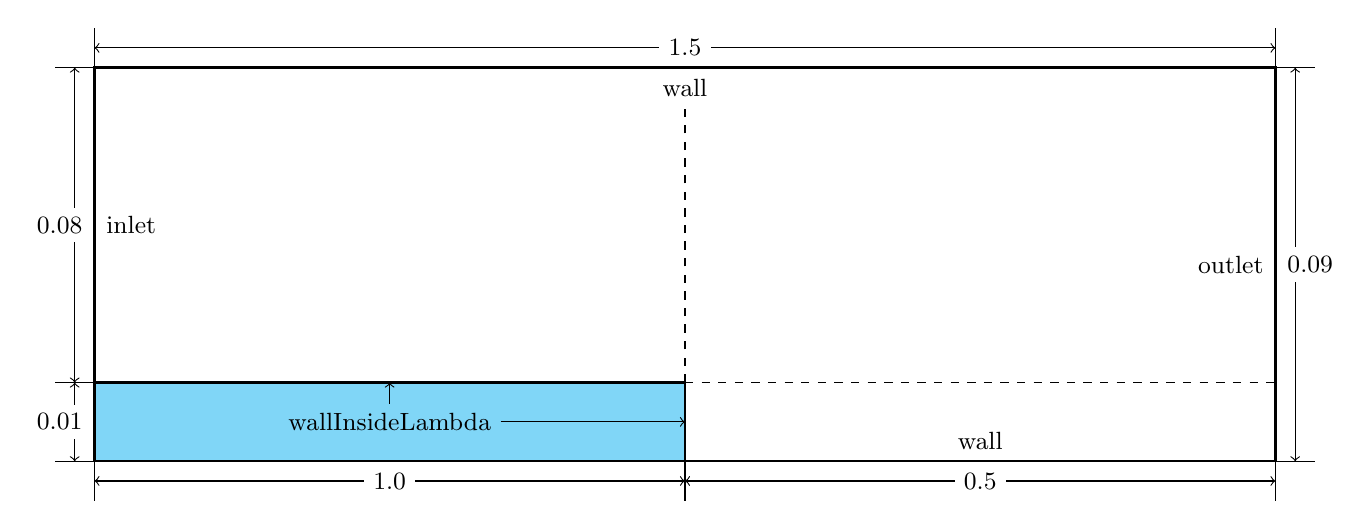
\begin{tikzpicture}
	%% domain base
	\draw[thick] (0, 0) rectangle (15, 5);
	\draw[thick, fill=cyan!50!white] (0, 0) rectangle (7.5, 1);

	%% block split
	\draw[dashed, thin] (7.5, 1) -- (7.5, 5);
	\draw[dashed, thin] (7.5, 1) -- (15, 1);

	%% measurement ticks
	\draw (-0.5, 0) -- (0, 0);
	\draw (-0.5, 1) -- (0, 1);
	\draw (-0.5, 5) -- (0, 5);

	\draw (0, 5) -- (0, 5.5);
	\draw (15, 5) -- (15, 5.5);

	\draw (15, 5) -- (15.5, 5);
	\draw (15, 0) -- (15.5, 0);

	\draw (0, 0) -- (0, -0.5);
	\draw (7.5, 0) -- (7.5, -0.5);
	\draw (15, 0) -- (15, -0.5);

	%% measurement lines
	\draw[<->] (-0.25, 0) -- (-0.25, 1);
	\draw[<->] (-0.25, 1) -- (-0.25, 5);

	\draw[<->] (0, 5.25) -- (15, 5.25);

	\draw[<->] (15.25, 0) -- (15.25, 5);

	\draw[<->] (7.5, -0.25) -- (15, -0.25);
	\draw[<->] (0, -0.25) -- (7.5, -0.25);

	%% measurements
	\node[anchor=east, fill=white, outer sep=1pt] at (0, 0.5) {\small 0.01};
	\node[anchor=east, fill=white, outer sep=1pt] at (0, 3) {\small 0.08};
	\node[anchor=south, fill=white, outer sep=1pt] at (7.5, 5) {\small 1.5};
	\node[anchor=west, fill=white, outer sep=1pt] at (15, 2.5) {\small 0.09};
	\node[anchor=north, fill=white, outer sep=1pt] at (11.25, 0) {\small 0.5};
	\node[anchor=north, fill=white, outer sep=1pt] at (3.75, 0) {\small 1.0};

	%% boundary conditions
	\node[anchor=center] (wil)  at (3.75, 0.5) {\small wallInsideLambda};
	\node[anchor=west, fill=white, outer sep=1pt] at (0, 3) {\small inlet};
	\node[anchor=north, fill=white, outer sep=1pt] at (7.5, 5) {\small wall};
	\node[anchor=east, fill=white, outer sep=1pt] at (15, 2.5) {\small outlet};
	\node[anchor=south, fill=white, outer sep=1pt] at (11.25, 0) {\small wall};

	%% wallInsideLambda pointers
	\draw[->] (wil.north) -- (3.75, 1);
	\draw[->] (wil.east) -- (7.5, 0.5);
\end{tikzpicture}

\end{document}
